% add. options: [seceqn,secthm,crcready,onecolumn]
\documentclass[sw]{iosart2x}

%\usepackage{dcolumn}
%\usepackage{endnotes}
\usepackage{booktabs}
\usepackage{tabulary}
\usepackage{csquotes}
\usepackage{siunitx}
%\usepackage{graphicx}
\usepackage{todonotes}
%\usepackage{natbib} % does not seem to work with ios 1
\renewcommand{\citet}{\cite}% citet is not defined without natbib
\renewcommand{\citep}{\cite}% citep is not defined without natbib
\setlength{\marginparwidth}{2.1cm}% enough space for todonotes
\usepackage{listings}
\lstset{language=SPARQL,breaklines=true}
%\usepackage{cleveref}
%%%%%%%%%%% End of definitions

\pubyear{2019}
\volume{0}
\firstpage{1}
\lastpage{1}

\begin{document}

\begin{frontmatter}

%\pretitle{}
\title{The SNIK Ontology of Hospital Information Management}
\runningtitle{The SNIK Ontology of Hospital Information Management}
%\subtitle{}

% Two or more authors:
\author[A]{\inits {K.}\fnms{Konrad} \snm{Höffner}\ead[label=e1]{konrad.hoeffner@imise.uni-leipzig.de}%
\thanks{Corresponding author. \printead{e1}.}},
\author[A]{\fnms{Franziska} \snm{Jahn}\ead[label=e2]{franziska.jahn@imise.uni-leipzig.de}},
\author[A]{\fnms{Birgit} \snm{Schneider}\ead[label=e3]{birgit.schneider@imise.uni-leipzig.de}},
\author[A]{\fnms{Anna} \snm{Lörke}\ead[label=e4]{anna.loerke@imise.uni-leipzig.de}},
\author[A]{\fnms{Thomas} \snm{Pause}\ead[label=e5]{thomas.pause@imise.uni-leipzig.de}},
\author[A]{\fnms{Alfred} \snm{Winter}\ead[label=e6]{alfred.winter@imise.uni-leipzig.de}}
\runningauthor{K. Höffner et al.}
\address[A]{Institute for Medical Informatics, Statistics and Epidemiology (IMISE),
\orgname{University of Leipzig}, \cny{Germany}\printead[presep={\\}]{e1,e2,e3,e4,e5,e6}}
%Medical Informatics, Management of Health Information Systemsi
%Härtelstraße 16--18, D-04107 Leipzig

\begin{abstract}
This paper describes the ontology of the \textbf{Semantic Network of Information Management in Hospitals} (SNIK).  
\end{abstract}


\begin{keyword}
\kwd{information management, information systems, hospital information management}
\end{keyword}

\end{frontmatter}

\begin{table}
\caption{}
\label{tab:namespaces}
\begin{tabular}{ll}
\toprule
\textbf{x}	&\textbf{y}\\
\midrule
\bottomrule
\end{tabular}
\end{table}


\section{Introduction}
Publishing textbook knowledge as Linked Data enables different ways of teaching.
The data is the result of 
The extraction effort includes 
The data is continously revised: users constantly report wrong or missing data in the visualization, which is then corrected, respectively revised, by the researchers of the project.

This paper describes the current state of digitalized Hospital Information Management textbook knowledge.

Using a data model of Information Management 
Depending on the learning style and information need of the student, several tools are available to cosnume that knowledge.


\section{Unsorted}

\begin{tabular*}{\columnwidth}{l}
Which components of a healthcare network are not healthcare institutions?\\
\begin{lstlisting}
SELECT ?x {bb:HealthCareNetwork meta:entityTypeComponent ?x.
  MINUS {?x rdfs:subClassOf* bb:HealthCareInstitution.}}
\end{lstlisting}\\
%bb:GovernmentalAuthority\\

How many functions is the CIO responsible for?\\
\begin{lstlisting}
SELECT COUNT(?f) {bb:ChiefInformationOfficer meta:isResponsibleForFunction ?f.}
\end{lstlisting}\\
%15\\

Do transinstitutional health information systems support telemicroscopy?\\
\begin{lstlisting}
ASK {bb:TransinstitutionalHealthInformationSystem meta:supports bb:Telemicroscopy.}
\end{lstlisting}
\end{tabular*}

\begin{tabulary}{\columnwidth}{lL}
\toprule
URL		&\url{http://www.snik.eu/ontology}\\
Version		&2018-10-10, 0.4.1\\
License		&CC BY-NC-SA 4.0\\
SPARQL Endpoint	&\url{http://www.snik.eu/sparql}\\
Visualization	&\url{http://www.snik.eu/graph}\\
RDF Browser	&\url{http://www.snik.eu/ontology}\\
Download	&\url{https://github.com/IMISE/snik-ontology/releases/download/0.8.0/snik-0.8.zip}\\
\# Triples	&\num{112747}\\
\# Classes	&\num{4729}\\
\# Properties	&\num{329}\\
\# Interlinks	&\num{713}\\
%Subontologies	&\url{http://www.snik.eu/ontology/bb}\\
%		&\url{http://www.snik.eu/ontology/ciox,}\\
%		&\url{http://www.snik.eu/ontology/ob}\\
%		&\url{http://www.snik.eu/ontology/he}\\
%		&\url{http://www.snik.eu/ontology/it4it}\\
\bottomrule
\end{tabulary}%The source code for the services is available at \url{https://github.com/imise}

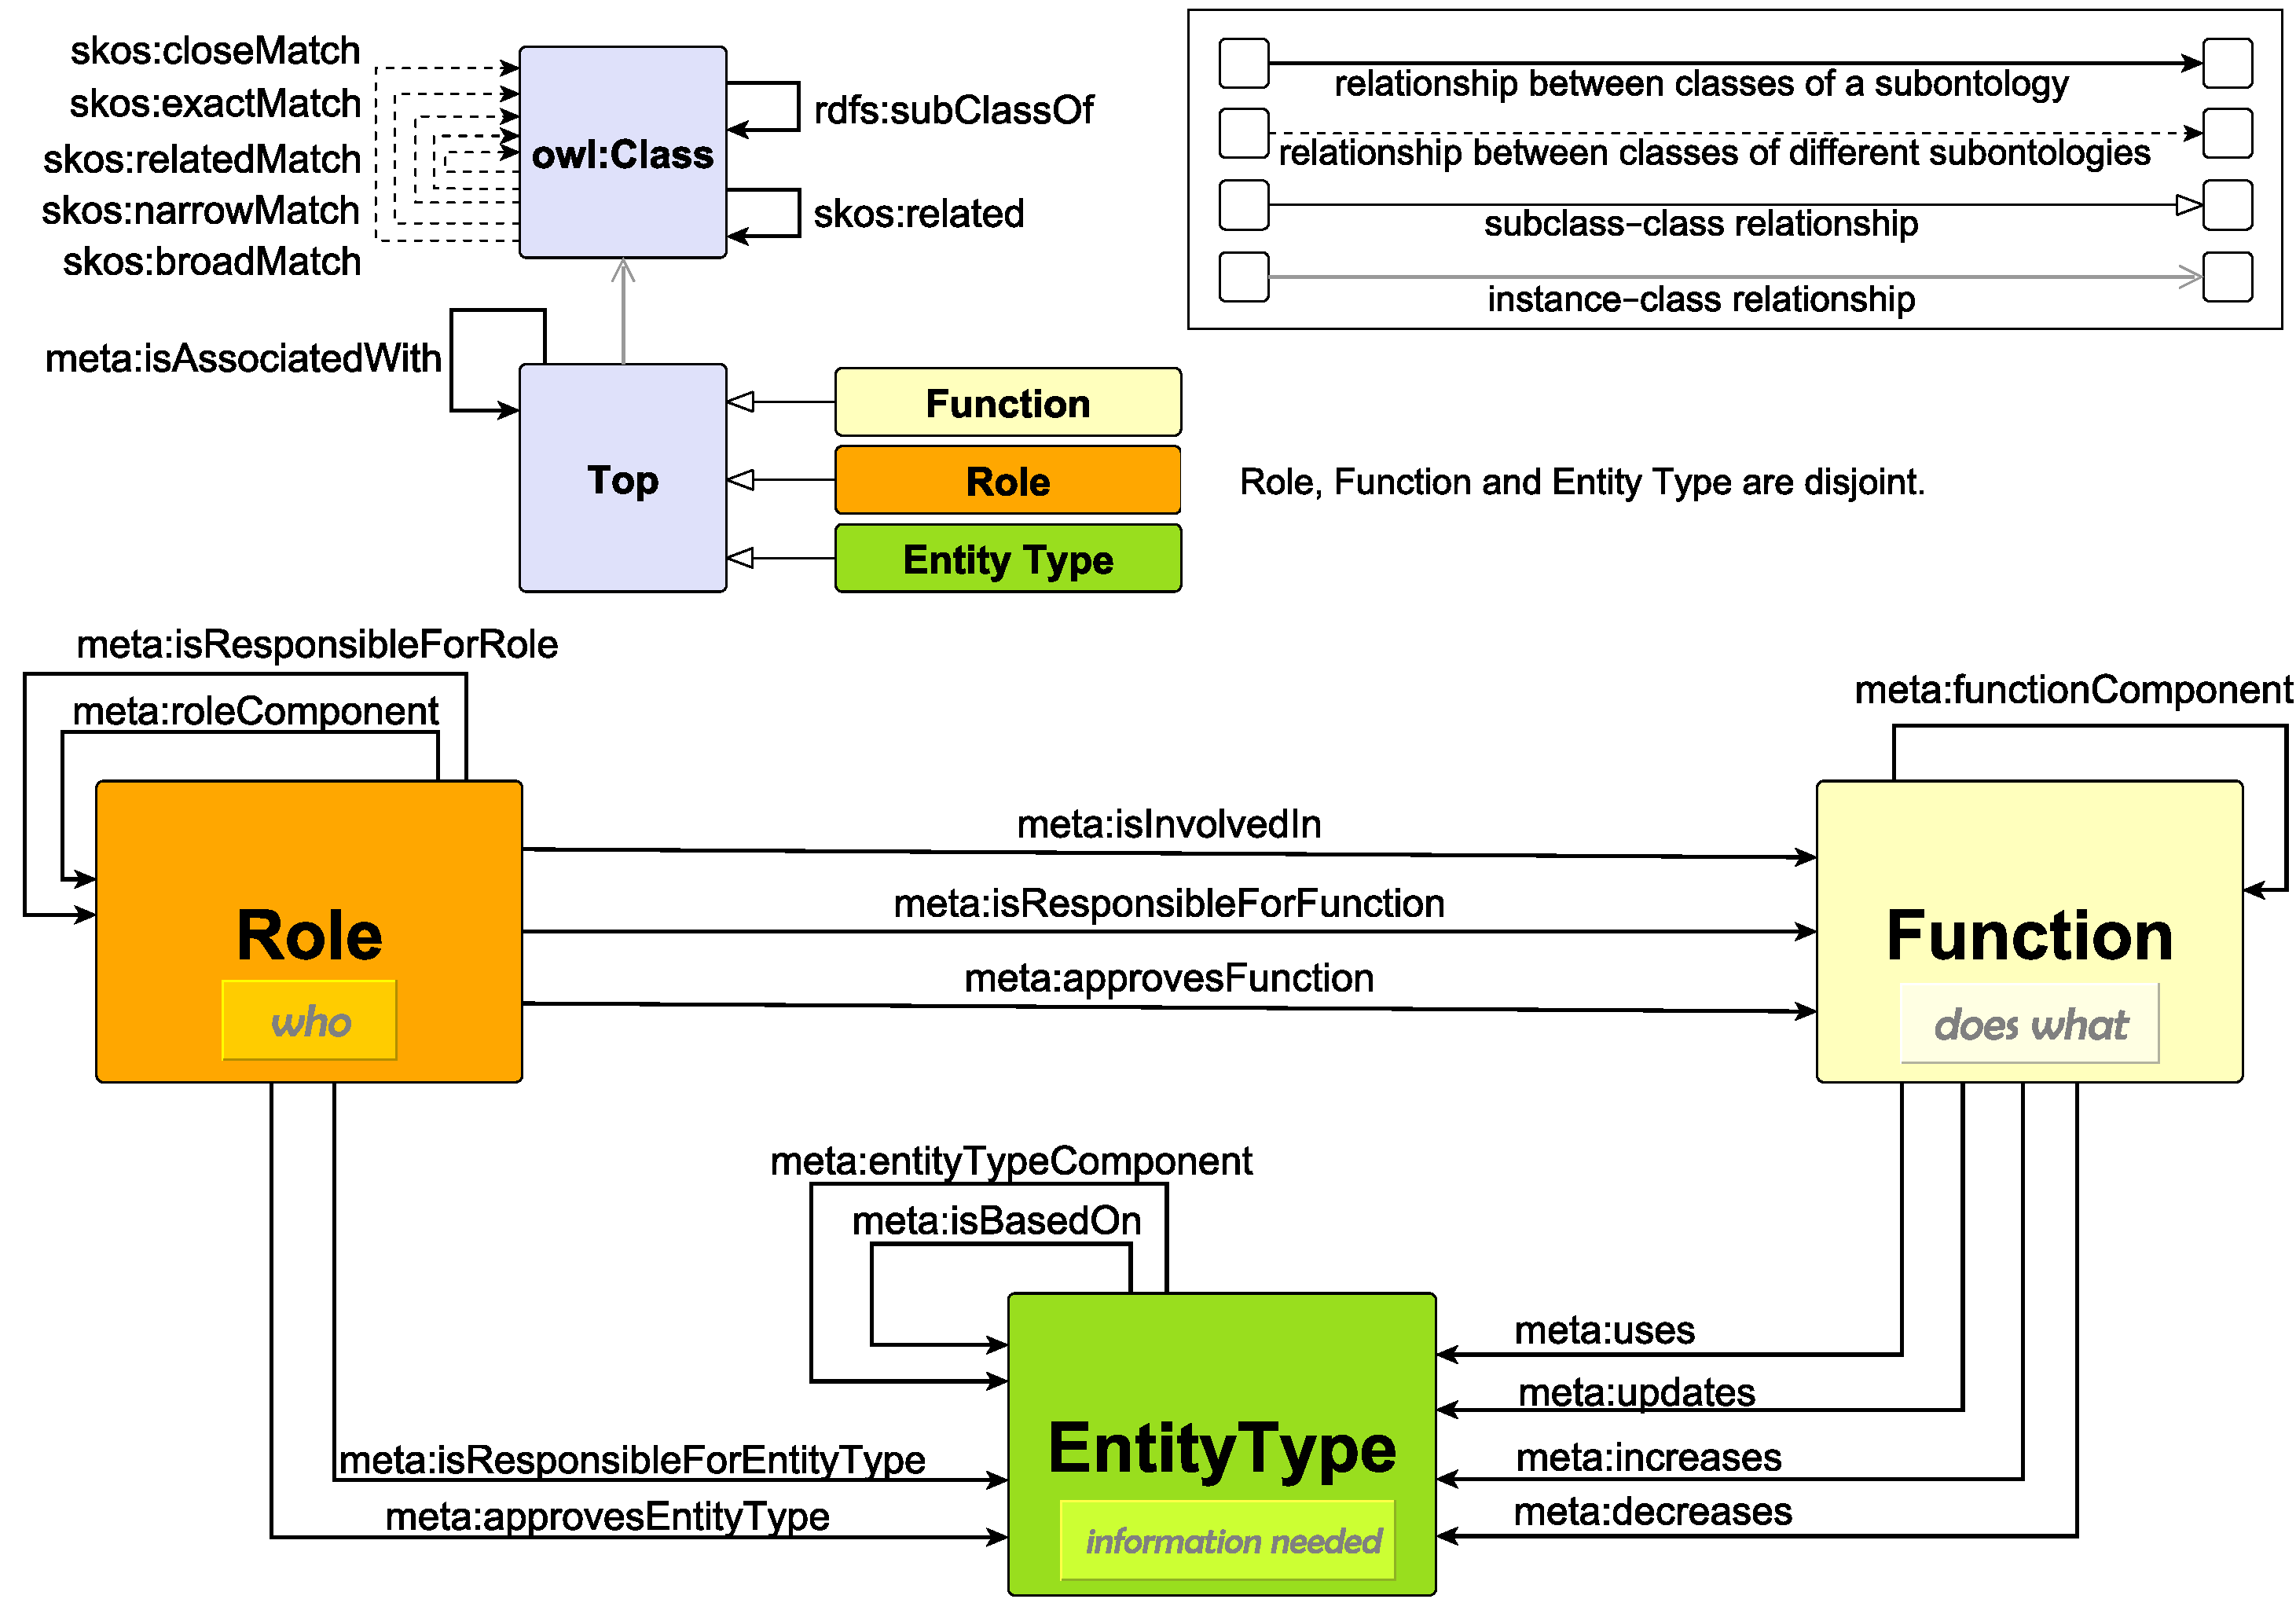
\includegraphics[width=\columnwidth]{img/metamodel9s.pdf}
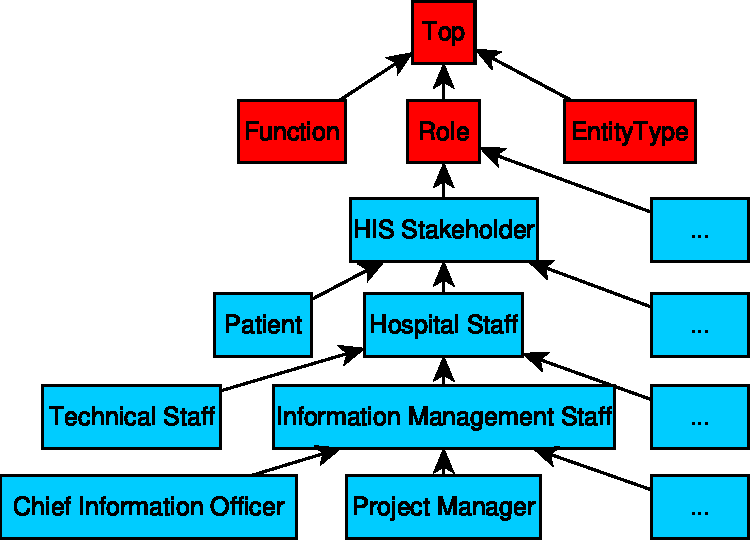
\includegraphics[width=\columnwidth]{img/hierarchy.pdf}
\begin{center}
\begin{tabular*}{0.96\columnwidth}{lll}
\toprule
\textbf{Ontology}				&\textbf{Prefix}&\textbf{Source}\\
\midrule
\url{http://www.snik.eu/ontology/meta}		&meta		&All Sources\\
\url{http://www.snik.eu/ontology/bb}		&bb		&Textbook~\cite{bb}\\
\url{http://www.snik.eu/ontology/ob}		&ob		&Textbook~\cite{ob}\\
\url{http://www.snik.eu/ontology/he}		&he		&Textbook~\cite{he}\\
\url{http://www.snik.eu/ontology/ciox}		&ciox		&CIO Interview\\
\url{http://www.snik.eu/ontology/it4it}		&it4it		&Standard~\cite{it4it}\\
\bottomrule
\end{tabular*}
\end{center}

\section{Sources}\label{sec:sources}
Three textbooks provide different views on the domain of Hospital Information Management:
\citet{bb} presents a broad view on \enquote{typical architectures of health information systems and their systematic strategic management}.
\citep{ob} concentrates on the \emph{tactical} management of information systems in general and on healthcare in particular.
The focus of tactical management lies on the planning and operation of projects.  
\citet{he} explains information management beyond the scope of healthcare. 
CIOX is based on an interview with the CIO of the Universitätsklinikum Leipzig.
IT4IT is based on the IT4IT standard.\todo{Sebastian: Was über Standards und IT4IT schreiben}

\section{Data Model}\label{sec:architecture}
\citet{domaene} contains an initial structure of the meta model.
\todo{Describe the meta model here}
The \textbf{Semantic Network of Information Management in Hospitals} (SNIK\footnote{Hospital means \enquote{Krankenhaus} in German.}) is a modular OWL 2 DL ontology.
The \enquote{Meta Model} defines three basic disjunctive classes and their possible relations: Roles (who), Function (does what) and Entity Types (and which information is therefore needed).
A set of modular subontologies define subclasses of those three classes and their relations as described by a certain knowledge source about information management in hospitals:
%from different sources:% three textbooks, an interview and a standard.

\section{Data Set Description}\label{sec:dsd}
The SNIK ontologies are available at \url{http://www.snik.eu/ontology/} under the Creative Commons Attribution-NonCommercial-ShareAlike 4.0 International license.

\section{Application}\label{sec:application}
The SNIK ontologies were initially intended~\citep{domaene} as the data source for \textbf{software to support hospital CIOs}:
(1) The requirements engineering decision support system TOREOnto~\citep{toreonto} and (2) the knowledge exploration and navigation visualization CIONo~\citep{ciono}.
While those applications were designed and prototypes were implemented, they were ultimately not integrated into the informational infrastructure of the Uniklinikum Leipzig.

Recent efforts focus on ontology assisted \textbf{teaching}. 
SNIK Graph~\citep{snikgraph}

\todo{verweis auf existierende papers}
\todo{benutzung durch braunschweig}
\todo{benutzung durch amsterdam}


\section{Acknowledgments}
We thank the publishers ... and ... for granting us permission to publish the subontologies based on the textbooks \citet{bb,ob,he} under an open license.
The SNIK project is supported by the DFG (German Research Foundation) under the grant numbers 1605/7-1 and 1387/8-1.
%\nocite{*} 
\bibliographystyle{ios1}
\bibliography{paper}

\end{document}
